%% ============================================================
%%  SIC-AI Capstone — Mid-Term Progress Report
%%  Speaker-Aware Noise Cancellation and Target Speech Enhancement
%%
%%  Build:  cd report && latexmk -pdf -interaction=nonstopmode main.tex
%% ============================================================
\documentclass[11pt,a4paper]{article}

\usepackage[T1]{fontenc}
\usepackage[utf8]{inputenc}
\usepackage{lmodern}
\usepackage[margin=2.4cm]{geometry}
\usepackage{microtype}
\usepackage{amsmath,amssymb}
\usepackage{graphicx}
\usepackage{booktabs,tabularx,array,multirow}
\usepackage{xcolor}
\newcolumntype{Y}{>{\raggedright\arraybackslash}X}
\usepackage{caption,subcaption}
\usepackage{enumitem}
\usepackage{float}
\usepackage{tikz}
\usetikzlibrary{positioning,arrows.meta,fit,calc}
\usepackage[numbers,sort&compress]{natbib}
\usepackage{fancyhdr}
\usepackage{setspace}
\usepackage[hidelinks]{hyperref}
\usepackage[nameinlink]{cleveref}

\setstretch{1.06}
\setlength{\parskip}{3.5pt}
\setlength{\parindent}{0pt}
\captionsetup{font=small,labelfont=bf,skip=4pt}
\setlist{itemsep=1.5pt,topsep=3pt}
\graphicspath{{figures/}}

% ---------- shortcuts ----------
\newcommand{\sisdr}{SI-SDR}
\newcommand{\sisdri}{SI-SDRi}
\newcommand{\spk}{\mathbf{e}}
\newcommand{\done}{\textbf{Completed}}
\newcommand{\partl}{\textbf{Partial}}
\newcommand{\pending}{\textbf{Pending}}
\newcommand{\inprog}{\textbf{In progress}}

% ---------- footer ----------
\pagestyle{fancy}
\fancyhf{}
\cfoot{\small\thepage}
\renewcommand{\headrulewidth}{0pt}

\begin{document}

%% ============================================================
%%  TITLE PAGE
%% ============================================================
\begin{titlepage}
\thispagestyle{empty}
\centering
{\Large\bfseries Samsung Innovation Campus\par}
\vspace{2mm}
{\large Enabling People Together\par}
\vspace{10mm}

\includegraphics[height=3.0cm]{tu_logo.png}\par
\vspace{8mm}
{\large Tribhuvan University\par}
\vspace{2mm}
{\large Pulchowk Campus\par}
\vspace{10mm}
{\large SIC-AI Capstone Project\par}
\vspace{2mm}
{\LARGE\bfseries Mid-Term Progress Report\par}
\vspace{12mm}
{\LARGE\bfseries Speaker-Aware Noise Cancellation\\ and Target Speech Enhancement\par}
\vspace{14mm}
{\large\bfseries Submitted By\par}
\vspace{3mm}
\begin{tabular}{@{}ll@{}}
Austina Aryal & (079BEI010)\\
Prashamsa Aryal & (079BEI024)\\
Sostika Shrestha & (079BEI041)
\end{tabular}
\vspace{10mm}

{\large\bfseries Submitted To\par}
\vspace{2mm}
{\large Arun Timilsena and Suresh Pokharel\par}
{\small Supervisors, SIC-AI Capstone Project\par}
\vfill
{\large November 2026 (Kartik 2083)\par}
\end{titlepage}
\setcounter{page}{2}

%% ============================================================
%%  ABSTRACT
%% ============================================================
\section*{Abstract}
This report presents the research, design, implementation, and evaluation of our SIC-AI capstone
project on target speaker extraction (TSE). The objective is to extract the voice of a specified
speaker from a single-channel speech mixture containing interfering speakers and background
noise, using a short enrollment recording of the target speaker as a reference.

We implemented and trained a speaker-conditioned Band-Split Recurrent Neural Network (BSRNN)
integrated with a frozen ECAPA-TDNN speaker encoder. The ECAPA-TDNN extracts a 192-dimensional
speaker embedding from the enrollment audio, which is incorporated into the separator through
speaker-feature addition and FiLM conditioning across eight dual-path layers. The resulting model
contains approximately 16.83 million parameters. It was trained on dynamically generated mixtures
of LibriSpeech speech and DEMAND environmental noise using a combined scale-invariant
signal-to-distortion ratio (SI-SDR) and multi-resolution STFT loss.

The model completed 100 training epochs, achieving its best validation SI-SDR improvement
(SI-SDRi) of 11.84\,dB at epoch~97, evaluated on unseen speakers. On the 1,200-mixture test set,
the epoch-97 checkpoint achieved an SI-SDR improvement of 11.6\,dB on non-clean mixtures and
increased STOI from 0.77 to 0.88, indicating improved speech intelligibility. A Whisper-based
evaluation also showed a reduction in word error rate from 38.3\% to 18.1\%. The model selected
the incorrect speaker in 7.7\% of interferer-containing mixtures, with most errors occurring when
enrollment recordings were short.

These results demonstrate that the implemented speaker-conditioned BSRNN can effectively extract
a target speaker from mixtures containing competing speech and environmental noise. The report
also discusses the system's limitations, including its non-causal architecture, and outlines
remaining work involving conditioning ablation, evaluation on unseen noise conditions, and CPU
inference measurements.

\newpage
\begingroup
\small
\setlength{\parskip}{0pt}
\tableofcontents
\endgroup
\newpage

%% ============================================================
%%  1. INTRODUCTION
%% ============================================================
\section{Introduction}
\label{sec:intro}

\subsection{Problem and motivation}
Conventional noise suppression removes environmental noise but treats every human voice as
signal. In a call or a meeting, a second person talking nearby is not noise in that sense, yet is
still unwanted. Target speaker extraction (TSE) handles this by conditioning the enhancement
network on an enrollment recording of the desired speaker, so that only that voice is kept
\cite{wang2019voicefilter, sato2024speakerbeamss}. Because the output is tied to one enrolled
speaker, TSE avoids the permutation problem of blind speech separation and does not need to know
how many speakers are present.

\subsection{Objectives}
The main objective of this project is to design, implement, and evaluate a deep-learning-based,
speaker-conditioned target-speaker extraction system that extracts a target speaker's speech from
single-channel mixtures containing interfering speakers and background noise, using a short
enrollment recording as a speaker reference. The specific objectives are:
\begin{enumerate}
  \item to design and implement a target-speaker extraction system that integrates a pretrained
        ECAPA-TDNN speaker encoder with a speaker-conditioned Band-Split Recurrent Neural Network
        (BSRNN) separator;
  \item to train and evaluate the system on speech mixtures containing competing speakers and
        environmental noise, using objective measures such as \sisdri, STOI and word error rate
        (WER);
  \item to study generalisation and robustness on unseen speakers and noise conditions, and to
        examine target-speaker selection errors under different enrollment conditions;
  \item to assess computational requirements and practical limitations, including parameter
        count, model size, inference efficiency and suitability for resource-constrained
        deployment; and
  \item to develop a reproducible training and evaluation framework covering dataset preparation,
        mixture generation, model training, checkpointing and systematic evaluation.
\end{enumerate}

\subsection{Scope and organisation of this report}
This report documents the completed data pipeline, the system architecture, the training and
evaluation methodology, the results obtained from the full 100-epoch run, and the main limitations
and remaining work. \Cref{sec:status} summarises progress at mid-term. \Cref{sec:method} describes
the end-to-end methodology, from data collection to evaluation. \Cref{sec:results} reports the
results. \Cref{sec:limits,sec:remaining} discuss limitations and the revised plan, and
\Cref{sec:conclusion} concludes.

\subsection{Progress at a glance}
\label{sec:status}
\Cref{tab:status} summarises the work completed at mid-term. All core components of the pipeline
are in place and the main model has finished training. The remaining items are ablation,
robustness testing and deployment-oriented work.

\begin{table}[htbp]
\centering\footnotesize
\caption{Status of project activities at mid-term.}
\label{tab:status}
\begin{tabularx}{\textwidth}{@{}>{\raggedright\arraybackslash}p{4.0cm} l Y@{}}
\toprule
\textbf{Activity} & \textbf{Status} & \textbf{Outcome / evidence}\\
\midrule
Literature and dataset survey & \done &
  Reviewed TSE, BSRNN, dual-path modelling, speaker embeddings and conditioning; selected
  LibriSpeech and DEMAND.\\
Data collection & \done &
  LibriSpeech \texttt{train-clean-100/360}, \texttt{dev-clean} and \texttt{test-clean};
  16 DEMAND environments.\\
Data preparation & \done &
  16\,kHz manifests, speaker-disjoint splits, VAD-cleaned enrollment banks and fixed
  validation/test mixtures (\Cref{sec:data,sec:prep}).\\
Mixture simulation & \done &
  Four scene types, SIR/SNR sampling, 4\,s training and 6\,s evaluation clips
  (\Cref{sec:mixture}).\\
Conv-TasNet baseline & \done &
  Causal baseline reached 5.90\,dB validation \sisdri{} at epoch 21; retained as a reference
  (\Cref{tab:convtasnet}).\\
Speaker encoder and conditioning & \done &
  Frozen ECAPA-TDNN, 192-d embeddings, additive and FiLM conditioning implemented
  (\Cref{sec:system}).\\
BSRNN separator & \done &
  16.83\,M parameters, 8 dual-path layers; 100 epochs completed, best validation \sisdri{}
  11.84\,dB at epoch 97 (\Cref{sec:results}).\\
Training pipeline & \done &
  Resumable training with checkpointing, fp16, gradient checkpointing and cached embeddings;
  no skipped batches in the final run.\\
Evaluation & \done &
  1200-mixture test evaluation, SI-SDR/STOI/PESQ with bootstrap intervals, scenario/SIR/SNR/noise
  breakdowns, speaker confusion, WER and efficiency (\Cref{sec:results}).\\
Ablation and robustness & \inprog &
  Conditioning ablation, unseen-noise evaluation, target-absent and enrollment studies
  (\Cref{sec:remaining}).\\
Deployment and documentation & \inprog &
  CPU benchmark, causal/compact variant, demo and final report (\Cref{sec:remaining}).\\
\bottomrule
\end{tabularx}
\end{table}

%% ============================================================
%%  2. METHODOLOGY
%% ============================================================
\section{Methodology and Workflow}
\label{sec:method}

\subsection{Overview}
The study follows a six-stage workflow: data collection, data preparation, mixture simulation,
model construction, training and evaluation. \Cref{fig:workflow} shows the complete flow. The
notebooks are treated as an execution record; the description below focuses on the method, the
data and the decisions that shaped the final system. Evaluation informs the discussion of model
behaviour, limitations and future improvements.

\begin{figure}[t]
\centering
\resizebox{0.90\textwidth}{!}{%
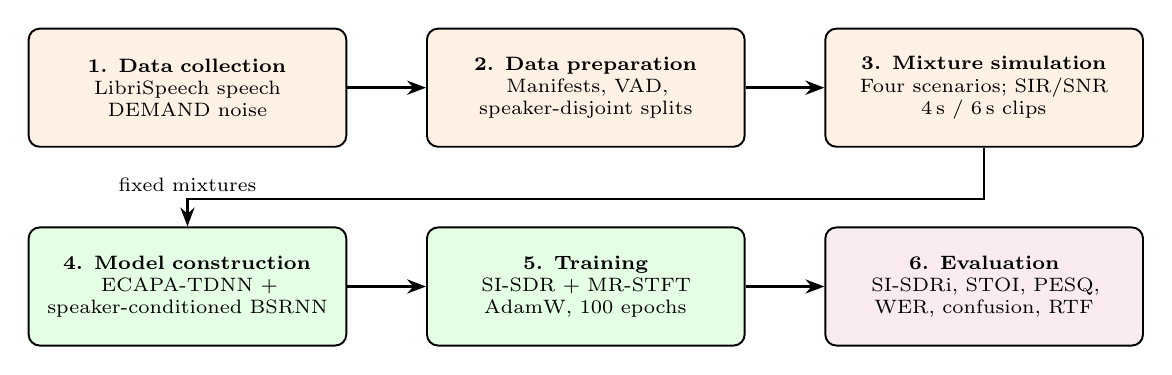
\begin{tikzpicture}[
  >=Stealth,
  stage/.style={draw, rounded corners=4pt, align=center, font=\scriptsize,
                minimum height=15mm, text width=3.8cm, line width=0.7pt},
  data/.style={stage, fill=orange!10},
  model/.style={stage, fill=green!10},
  eval/.style={stage, fill=purple!8},
  ar/.style={-{Stealth[length=2.4mm]}, line width=0.9pt},
  far/.style={-{Stealth[length=2.4mm]}, line width=0.8pt, dashed, gray}
]
\node[data] (collect) {\textbf{1. Data collection}\\LibriSpeech speech\\DEMAND noise};
\node[data, right=of collect] (prep) {\textbf{2. Data preparation}\\Manifests, VAD,\\speaker-disjoint splits};
\node[data, right=of prep] (mix) {\textbf{3. Mixture simulation}\\Four scenarios; SIR/SNR\\4\,s / 6\,s clips};
\node[model, below=of collect] (arch) {\textbf{4. Model construction}\\ECAPA-TDNN +\\speaker-conditioned BSRNN};
\node[model, right=of arch] (train) {\textbf{5. Training}\\SI-SDR + MR-STFT\\AdamW, 100 epochs};
\node[eval, right=of train] (ev) {\textbf{6. Evaluation}\\SI-SDRi, STOI, PESQ,\\WER, confusion, RTF};
\draw[ar] (collect) -- (prep);
\draw[ar] (prep) -- (mix);
\draw[ar] (mix.south) -- ++(0,-0.65) -| node[pos=0.55, above, font=\scriptsize]{fixed mixtures} (arch.north);
\draw[ar] (arch) -- (train);
\draw[ar] (train) -- (ev);
\end{tikzpicture}%
}
\caption{Six-stage research workflow from data collection through evaluation.}
\label{fig:workflow}
\end{figure}

\subsection{Data collection}
\label{sec:data}
Two public corpora are used. \textbf{LibriSpeech} \cite{panayotov2015librispeech} supplies clean
read English at 16\,kHz. Training uses \texttt{train-clean-100} and \texttt{train-clean-360}
(251 + 921 = 1172 speakers); validation uses \texttt{dev-clean} (40 speakers) and testing uses
\texttt{test-clean} (40 speakers). Validation and test speakers never appear in training, so these
sets measure generalisation to unseen voices.

\textbf{DEMAND} \cite{thiemann2013demand} supplies real environmental recordings at 16\,kHz. It
contains domestic, outdoor and transport scenes such as kitchens, living rooms, parks, streets,
offices, restaurants, buses, cars and metro stations. Sixteen environments were used. In this
report, the symbol $n$ always
denotes this non-speech environmental noise. It is not the interfering talker: the interfering
speaker is a separate speech source drawn from LibriSpeech and is treated as interference, not as
noise.

\Cref{tab:corpora} summarises the roles, subsets and clip lengths. The validation set contains 300
fixed mixtures (seed 1234) and the test set contains 1200 fixed mixtures (seed 4321).

\begin{table}[htbp]
\centering\footnotesize
\caption{Speech and noise corpora used in the study.}
\label{tab:corpora}
\begin{tabularx}{\textwidth}{@{}l l l r c@{}}
\toprule
\textbf{Corpus} & \textbf{Role} & \textbf{Subset / environment} & \textbf{Speakers} & \textbf{Clip}\\
\midrule
LibriSpeech & Target and interferer speech & \texttt{train-clean-100} & 251 & 4\,s\\
LibriSpeech & Target and interferer speech & \texttt{train-clean-360} & 921 & 4\,s\\
LibriSpeech & Validation speech & \texttt{dev-clean} & 40 & 6\,s\\
LibriSpeech & Test speech & \texttt{test-clean} & 40 & 6\,s\\
DEMAND & Environmental noise $n$ & 16 environments & -- & 4/6\,s\\
\bottomrule
\end{tabularx}
\end{table}

\subsection{Data preparation:}
\label{sec:prep}
The raw corpora are not used directly. The following preparation steps are applied once and then
reused by every experiment.
\begin{enumerate}
  \item \textbf{Verification and formatting.} Each LibriSpeech subset is checked against its
        expected speaker count and converted to 16\,kHz mono. Utterances shorter than the target
        crop are excluded or padded with silence by the loader.
  \item \textbf{Manifests.} A manifest row stores the utterance identifier, speaker identifier,
        file path and duration. Separate manifests are built for training, validation and test
        speech.
  \item \textbf{Speaker-disjoint splits.} Training, validation and test speakers are disjoint.
        The fixed validation and test mixture manifests are generated once so that every model
        is compared on exactly the same mixtures.
  \item \textbf{Noise partition.} Each DEMAND recording is split by time: the first 80\% for
        training, the next 10\% for validation and the final 10\% for testing. No noise audio is
        shared across splits, but the same 16 environments appear in all three.
  \item \textbf{Enrollment preparation.} Enrollment audio is cleaned with a voice activity
        detector (VAD), concatenated and cut to a random duration. Ten enrollment recipes are
        stored for each training speaker and six for each validation and test speaker. The
        mixture's own target utterance is never used in its enrollment.
  \item \textbf{Embedding cache.} ECAPA-TDNN embeddings are pre-computed for all enrollment
        recipes (about 11.7k training embeddings) so that the speaker encoder costs no GPU time or
        memory during training.
\end{enumerate}

\paragraph{Voice activity detection.}
Let $x[n]$ be the enrollment waveform, where $n$ indexes audio samples. Frames of $L=400$ samples
(25\,ms at 16\,kHz) are taken every $H=160$ samples (10\,ms); $t$ indexes the frame. The frame
energy and its decibel value are
\begin{equation}
  E_t=\frac{1}{L}\sum_{n=0}^{L-1}x^2[tH+n],
  \qquad
  E_t^{\mathrm{dB}}=10\log_{10}(E_t+\epsilon).
\end{equation}
where $\epsilon$ is a small positive constant that prevents $\log(0)$. The speech level is
estimated from the 95th percentile,
$E_{\mathrm{ref}}=P_{95}(\{E_t^{\mathrm{dB}}\})$, where $P_{95}$ denotes the value below which
95\% of the frame-energy values fall. A frame is marked voiced when
\begin{equation}
  v_t=
  \begin{cases}
    1, & E_t^{\mathrm{dB}}\ge \tau,\\
    0, & \text{otherwise},
  \end{cases}
  \qquad
  \tau=\max\left(E_{\mathrm{ref}}-30\,\mathrm{dB},\;-55\,\mathrm{dB}\right).
  \label{eq:vad}
\end{equation}
where $v_t\in\{0,1\}$ is the voiced/unvoiced indicator and $\tau$ is the adaptive energy
threshold; the fixed $-55$\,dB term is the minimum threshold. A 10-frame hangover retains a frame
if it or any of the preceding 10 frames is voiced:
\begin{equation}
  \tilde{v}_t=\max_{k=0,\ldots,10} v_{t-k}.
\end{equation}
where $\tilde v_t$ is the hangover-smoothed voice indicator and $k$ indexes previous frames. The
retained frames from several utterances of the same speaker are concatenated and truncated
to $d\in\{2,3,5,8,12\}$\,s with probabilities $0.15,0.20,0.30,0.20,0.15$. The resulting waveform
is passed to the frozen ECAPA-TDNN. The same VAD is used for the cached enrollment banks and for
a user-supplied enrollment recording at inference time.

\subsection{Mixture simulation}
\label{sec:mixture}
Training data are generated on the fly. Each scene contains a target $s_t$, optionally an
interfering talker $s_i$, and optionally environmental noise $n$. The two speech sources are
different LibriSpeech speakers. The mixture is
\begin{equation}
  x=s_t+\alpha s_i+\beta n .
  \label{eq:mixture}
\end{equation}
Let $P_s$, $P_i$ and $P_n$ be the mean powers of the target, interferer and noise, and let
$P_{s+\alpha i}$ denote the power of the speech component $s_t+\alpha s_i$. The target-to-
interferer ratio (SIR) and speech-to-noise ratio (SNR) are defined as
\begin{equation}
  \mathrm{SIR}=10\log_{10}\frac{P_s}{\alpha^2P_i},
  \qquad
  \mathrm{SNR}=10\log_{10}\frac{P_{s+\alpha i}}{\beta^2P_n},
\end{equation}
If a component is absent, its scale is set to zero and the corresponding ratio is not applicable.
SIR is sampled uniformly from
$[-5,5]$\,dB and SNR from $[-5,15]$\,dB. The mixture level is drawn from $[-35,-15]$\,dBFS and
passed through a peak limiter at 0.99. Training clips last 4\,s and evaluation clips 6\,s.

\Cref{tab:scenarios} lists the four scene types. With probability 0.5 the interferer covers only
30--100\% of the clip at a random offset. One model therefore learns target extraction, plain
denoising and leaving clean speech untouched.

\begin{table}[htbp]
\centering\footnotesize
\caption{Configured mixture categories. The probabilities sum to one. Here $n$ is environmental
noise, not an interfering talker.}
\label{tab:scenarios}
\begin{tabularx}{\textwidth}{@{}l c l Y@{}}
\toprule
\textbf{Scenario} & \textbf{Probability} & \textbf{Components} & \textbf{Purpose}\\
\midrule
\texttt{speech\_noise} & 0.45 & $s_t+\alpha s_i+\beta n$ &
  Joint competing-speech and noise suppression.\\
\texttt{speech} & 0.25 & $s_t+\alpha s_i$ &
  Speaker selectivity without environmental noise.\\
\texttt{noise} & 0.25 & $s_t+\beta n$ &
  Conventional denoising while preserving speaker identity.\\
\texttt{clean} & 0.05 & $s_t$ &
  Clean reference/control; tests that clean speech is left intact.\\
\bottomrule
\end{tabularx}
\end{table}

\subsection{System architecture:}
\label{sec:system}
\paragraph{Overview.}
Given the mixture $x$ and an enrollment recording $x_e$ of the target, the system estimates the
target speech as
\begin{equation}
  \hat{s}_t=\mathrm{iSTFT}\Big(M\odot \mathrm{STFT}(x)\Big),
  \qquad
  M=F\big(\mathrm{STFT}(x),\,g(f_{\mathrm{enc}}(x_e))\big),
\end{equation}
where $\hat{s}_t$ is the estimated target waveform, $x$ is the mixture, $x_e$ is the enrollment
waveform, $M$ is the complex time--frequency mask, $\odot$ denotes element-wise multiplication,
and STFT/iSTFT are the short-time Fourier transform and its inverse. The frozen speaker encoder
is $f_{\mathrm{enc}}$, $g$ is a projection network, and $F$ is the separator. \Cref{fig:arch}
shows the complete architecture. The enrollment branch and the mixture branch are separate until
the speaker vector is injected into the separator.

\begin{figure}[t]
\centering
\resizebox{\textwidth}{!}{%
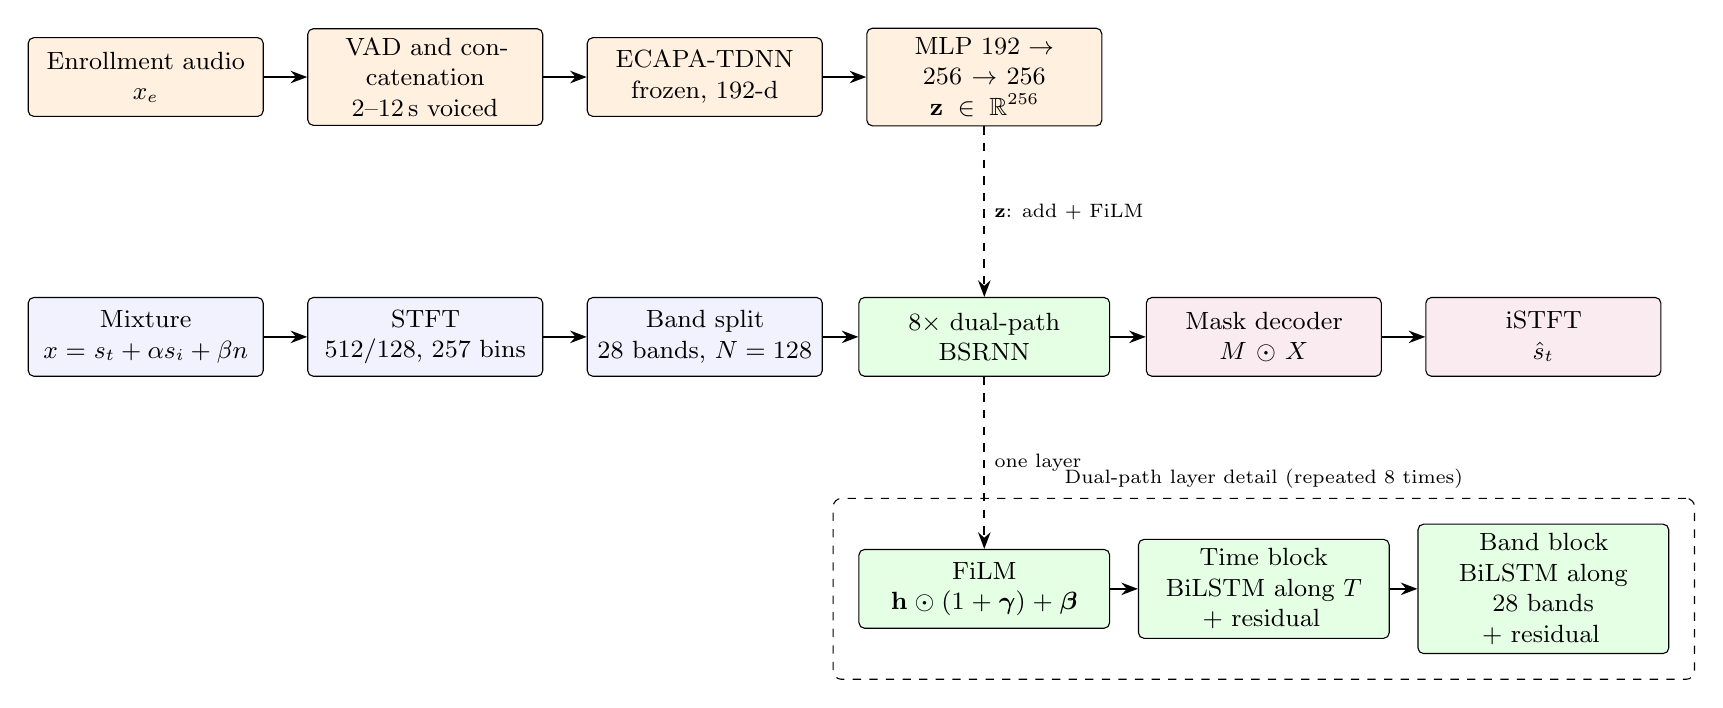
\begin{tikzpicture}[
  >=Stealth,
  box/.style={draw, rounded corners=2pt, align=center, font=\small,
              minimum height=10mm, text width=2.75cm, fill=blue!5},
  spk/.style={draw, rounded corners=2pt, align=center, font=\small,
              minimum height=10mm, text width=2.75cm, fill=orange!12},
  net/.style={draw, rounded corners=2pt, align=center, font=\small,
              minimum height=10mm, text width=2.95cm, fill=green!10},
  dec/.style={draw, rounded corners=2pt, align=center, font=\small,
              minimum height=10mm, text width=2.75cm, fill=purple!8},
  ar/.style={-{Stealth[length=2.1mm]}, thick},
  dar/.style={-{Stealth[length=2.1mm]}, thick, dashed}
]
% enrollment branch
\node[spk] (enr)  at (0,3.3) {Enrollment audio\\$x_e$};
\node[spk] (vad)  at (3.55,3.3) {VAD and concatenation\\2--12\,s voiced};
\node[spk] (ecapa) at (7.10,3.3) {ECAPA-TDNN\\frozen, 192-d};
\node[spk] (mlp)  at (10.65,3.3) {MLP $192\!\to\!256\!\to\!256$\\$\mathbf{z}\in\mathbb{R}^{256}$};
% signal branch
\node[box] (mix)   at (0,0) {Mixture\\$x=s_t+\alpha s_i+\beta n$};
\node[box] (stft)  at (3.55,0) {STFT\\512/128, 257 bins};
\node[box] (band)  at (7.10,0) {Band split\\28 bands, $N=128$};
\node[net] (bsrnn) at (10.65,0) {8$\times$ dual-path\\BSRNN};
\node[dec] (mask)  at (14.20,0) {Mask decoder\\$M\odot X$};
\node[dec] (istft) at (17.75,0) {iSTFT\\$\hat{s}_t$};
% detail row
\node[net] (film) at (10.65,-3.2) {FiLM\\$\mathbf{h}\odot(1+\boldsymbol\gamma)+\boldsymbol\beta$};
\node[net] (time) at (14.20,-3.2) {Time block\\BiLSTM along $T$\\+ residual};
\node[net] (freq) at (17.75,-3.2) {Band block\\BiLSTM along 28 bands\\+ residual};
% arrows
\draw[ar] (enr) -- (vad);
\draw[ar] (vad) -- (ecapa);
\draw[ar] (ecapa) -- (mlp);
\draw[ar] (mix) -- (stft);
\draw[ar] (stft) -- (band);
\draw[ar] (band) -- (bsrnn);
\draw[ar] (bsrnn) -- (mask);
\draw[ar] (mask) -- (istft);
\draw[dar] (mlp.south) -- (bsrnn.north)
  node[midway, right, font=\scriptsize]{$\mathbf{z}$: add + FiLM};
\draw[dar] (bsrnn.south) -- (film.north)
  node[midway, right, font=\scriptsize]{one layer};
\draw[ar] (film) -- (time);
\draw[ar] (time) -- (freq);
\node[draw, dashed, rounded corners=3pt, fit=(film)(freq), inner sep=3.2mm,
      label={[font=\scriptsize]above:Dual-path layer detail (repeated 8 times)}] {};
\end{tikzpicture}%
}
\caption{Speaker-conditioned BSRNN. The upper branch computes the speaker vector
$\mathbf{z}$ from the enrollment recording. The lower branch computes a complex mask from the
mixture. $\mathbf{z}$ is added once to the band features and is also used by FiLM inside every
dual-path layer. The dashed box shows one dual-path layer: a time block followed by a band
block, each with a residual connection.}
\label{fig:arch}
\end{figure}

\paragraph{Front end and band split.}
Audio is processed at 16\,kHz. The waveform is divided by its standard deviation, and the output
is multiplied back, so the network sees level-independent input. An STFT with a 512-point Hann
window (32\,ms) and a 128-sample hop (8\,ms) gives 257 complex bins per frame; a 4\,s training clip
yields 501 frames. STFT, iSTFT and the loss are computed in fp32 even under mixed precision.

The 257 bins are grouped into 28 non-uniform bands: 8 bands of 125\,Hz below 1\,kHz, 12 bands of
250\,Hz between 1 and 4\,kHz, and 8 bands of 500\,Hz between 4 and 8\,kHz. The last band takes the
one leftover bin. For band $b$, the real and imaginary parts are layer-normalised and linearly
projected to $N=128$ features:
\begin{equation}
  \mathbf{h}_b=\mathrm{LN}\!\left(\left[\Re X_b;\Im X_b\right]\right)W_b,
  \qquad
  H=[\mathbf{h}_1,\ldots,\mathbf{h}_{28}]\in\mathbb{R}^{B\times28\times T\times128}.
\end{equation}
Here $X_b$ is the STFT restricted to band $b$, $\Re$ and $\Im$ denote its real and imaginary
parts, $[\,;\,]$ concatenates them, $\mathrm{LN}$ is layer normalisation, $W_b$ is the learned
projection matrix for band $b$, $B$ is batch size, and $T$ is the number of time frames.
The fine low-frequency resolution follows the harmonic structure of speech; the coarser
high-frequency bands cost less and carry less formant information.

\paragraph{Speaker branch and conditioning.}
The enrollment audio is cleaned with the VAD of \Cref{eq:vad} and cut to 2--12\,s as described in
\Cref{sec:prep}. A frozen SpeechBrain ECAPA-TDNN (\texttt{spkrec-ecapa-voxceleb})
\cite{ravanelli2021speechbrain,desplanques2020ecapa} maps the enrollment to a 192-dimensional
embedding. The embedding is L2-normalised and passed through a small MLP
($192\to256\to256$, PReLU) to obtain $\mathbf{z}\in\mathbb{R}^{256}$.

The speaker vector enters the separator in two places. First, it is linearly projected to $N$
dimensions and added once to the band features before the first layer:
\begin{equation}
  H\leftarrow H+W_a\mathbf{z},
  \qquad W_a\in\mathbb{R}^{N\times256}.
\end{equation}
Here $\mathbf{z}\in\mathbb{R}^{256}$ is the projected speaker embedding, $W_a$ maps it to the
band-feature dimension, and the addition is broadcast over bands and time frames.
Second, every dual-path layer computes a per-channel scale and shift,
\begin{equation}
  [\boldsymbol\gamma,\boldsymbol\beta]=W_\ell\mathbf{z}+\mathbf{b}_\ell,
  \qquad
  \mathbf{h}'=\mathbf{h}\odot(1+\boldsymbol\gamma)+\boldsymbol\beta,
  \label{eq:film}
\end{equation}
where $\mathbf{h}$ is a feature vector, $\boldsymbol\gamma$ and $\boldsymbol\beta$ are the
per-channel scale and shift, and $W_\ell\in\mathbb{R}^{2N\times256}$ and $\mathbf{b}_\ell$ are
learned layer-specific parameters. The FiLM weights and bias are zero-initialised, so
training starts from an unconditioned BSRNN and learns to use the speaker cue gradually.

\paragraph{Dual-path layers and mask decoder.}
Each of the eight layers applies FiLM, then a time block and a band block, both with residual
connections:
\begin{align}
  \mathbf{h} &\leftarrow \mathbf{h}+\mathrm{BiLSTM}_{T}\!\left(\mathrm{LN}(\mathbf{h})\right),\\
  \mathbf{h} &\leftarrow \mathbf{h}+\mathrm{BiLSTM}_{B}\!\left(\mathrm{LN}(\mathbf{h})\right).
\end{align}
Here $\mathbf{h}$ is the current feature tensor, $\mathrm{LN}$ is layer normalisation, and the
subscripts $T$ and $B$ indicate the time and band BiLSTMs. The time block runs along $T$ for every band and gives long-range temporal context. The band
block runs along the 28 bands for every frame and models cross-frequency structure at the low cost
of a 28-step sequence.

The decoder is applied per band: LayerNorm, $\mathrm{Linear}(N,4N)$, Tanh,
$\mathrm{Linear}(4N,4\cdot\text{bins})$ and a GLU \cite{dauphin2017glu}, which produces a real and
an imaginary mask value for every bin. The mask is unbounded and complex, so it can change phase
as well as magnitude:
\begin{equation}
  \hat{S}(t,f)=M(t,f)X(t,f).
\end{equation}
Here $X(t,f)$ is the mixture STFT at time frame $t$ and frequency bin $f$, $M(t,f)$ is the
complex mask, and $\hat S(t,f)$ is the estimated target STFT.
With $N=128$, LSTM hidden size 256 and 8 layers, the model has \textbf{16.83\,M parameters} and
needs 23.87\,GMACs for a 6\,s clip (\Cref{sec:eff}).

\subsection{Training procedure}
\label{sec:training}
For an estimate $\hat{s}$ and reference $s$, scale-invariant SDR \cite{leroux2019sdr} is
\begin{equation}
  \mathrm{SI\text{-}SDR}(\hat{s},s)=10\log_{10}\frac{\|\alpha s\|^2}{\|\alpha s-\hat{s}\|^2},
  \qquad
  \alpha=\frac{\langle\hat{s},s\rangle}{\|s\|^2},
  \label{eq:sisdr}
\end{equation}
Here $s$ is the clean reference, $\hat{s}$ is the estimate, $\alpha$ is the optimal scale factor,
$\langle\cdot,\cdot\rangle$ is the inner product, and $\|\cdot\|$ is the Euclidean norm.
computed after removing the mean of each signal. The training loss combines it with a
multi-resolution STFT loss \cite{yamamoto2020pwg}:
\begin{equation}
  \mathcal{L}=-\,w_1\,\mathbb{E}\big[\min(\mathrm{SI\text{-}SDR},\,30\,\mathrm{dB})\big]
  + w_2\,\mathcal{L}_{\text{MR-STFT}},
  \qquad w_1=1,\; w_2=5 .
  \label{eq:loss}
\end{equation}
$\mathcal{L}$ is the total training loss, $\mathbb{E}$ denotes the batch mean, $w_1$ and $w_2$
are loss weights, and $\mathcal{L}_{\text{MR-STFT}}$ is the multi-resolution spectral loss. It
sums spectral-convergence and log-magnitude terms at three
resolutions (window, hop) = (512,128), (1024,256) and (2048,512). The 30\,dB clamp stops
near-perfect examples, such as the clean scenario, from dominating the gradient.

\begin{table}[H]
\centering\footnotesize
\caption{Training configuration of the main run.}
\label{tab:hparams}
\begin{tabularx}{\textwidth}{@{}>{\raggedright\arraybackslash}p{3.5cm} Y@{}}
\toprule
Item & Value\\
\midrule
Model & BSRNN, $N=128$, hidden 256, 8 layers, 28 bands (16.83\,M parameters)\\
Optimiser & AdamW \cite{loshchilov2019adamw}, weight decay 0.01\\
Learning rate & 2000-step linear warm-up to $5\times10^{-4}$, cosine decay \cite{loshchilov2017sgdr}
  to $10^{-5}$ over 100k steps\\
Batch & 8 clips $\times$ 4\,s\\
Epoch definition & 1000 steps (data generated on the fly); 100 epochs = 100k steps = 800k scenes\\
Gradient clipping & global norm 5.0\\
Precision & fp16 autocast with GradScaler \cite{micikevicius2018mixed}; STFT, iSTFT and loss in fp32\\
Memory saving & Gradient checkpointing \cite{chen2016checkpointing} on every dual-path layer\\
Safety & Non-finite-loss batches are skipped and counted (none were skipped in the final run)\\
Checkpointing & \texttt{\_last.pt} every epoch (model, optimiser, scaler, log); \texttt{\_best.pt}
  on best validation \sisdri\\
Outcome & 100 epochs completed; best validation \sisdri{} 11.84\,dB at epoch 97\\
Hardware & NVIDIA L4 (Google Colab)\\
Speed & 0.99\,s/step, peak GPU memory 3.2\,GiB; about 17.5\,min/epoch after the resume; about
  36\,h in total\\
\bottomrule
\end{tabularx}
\end{table}

\subsection{Evaluation protocol}
\label{sec:eval}
The system is evaluated on the fixed 1200-mixture test set (40 unseen speakers) and on the
300-mixture validation set. The main metrics are:
\begin{itemize}
  \item \textbf{\sisdri} in dB, the difference between output and input \sisdr:
        $\mathrm{SI\text{-}SDRi}=\mathrm{SI\text{-}SDR}(\hat{s}_t,s_t)
        -\mathrm{SI\text{-}SDR}(x,s_t)$;
  \item \textbf{STOI} \cite{taal2011stoi}, a predicted intelligibility score in $[0,1]$;
  \item \textbf{wideband PESQ} \cite{itu2007p8622}, a perceptual quality score;
  \item \textbf{WER} from Whisper \texttt{small.en} \cite{radford2023whisper}, computed with
        \texttt{jiwer} against Whisper's transcript of the clean target;
  \item \textbf{speaker confusion}: the output is embedded with ECAPA-TDNN and counted as confused
        when its cosine similarity to the interferer exceeds its similarity to the target;
  \item \textbf{efficiency}: parameter count, GMACs, offline real-time factor (RTF) and peak GPU
        memory.
\end{itemize}
Means are reported with 95\% bootstrap confidence intervals (5000 resamples, seed 0). The 65
clean-scenario test items are excluded from the headline \sisdri{} because their input \sisdr{} is
about 105\,dB; including them produces a large negative ``improvement'' that is a metric artefact,
not a quality problem. Results are also broken down by scenario, SIR, SNR and noise environment.

\subsection{Design evolution}
The final design was reached through one main modelling change. The first separator studied was a
causal Conv-TasNet \cite{luo2019convtasnet} with $N=512$, $H=512$, film2 conditioning, 3\,s
segments, batch 3 with gradient accumulation 2 and learning rate $10^{-3}$. Its best saved
checkpoint was epoch~21 with a validation \sisdri{} of 5.90\,dB; a 20-clip check gave 3.88\,dB on
training voices and 3.60\,dB on held-out voices and noise. The BSRNN separator reached 11.84\,dB
on the same validation set, so the final system uses BSRNN. The change was deliberately limited:
the front end, loss, optimiser and evaluation protocol were kept, while the separator was replaced
and the STFT hop was reduced from 160 to 128 samples (10\,ms to 8\,ms) for finer time resolution.
The Conv-TasNet configuration is retained in \Cref{tab:convtasnet} as a documented baseline.

%% ============================================================
%%  4. RESULTS
%% ============================================================
\section{Results:}
\label{sec:results}

Training finished all 100 epochs. The best validation checkpoint
(\texttt{tse\_bsrnn\_big\_best.pt}) was reached at \textbf{epoch~97}, with a validation \sisdri{}
of \textbf{11.84\,dB} on unseen speakers. The fixed test set contains 1200 mixtures from 40
unseen speakers. All results in this section use the epoch-97 checkpoint.\footnote{The checkpoint
file stores the zero-based epoch index 96, which corresponds to epoch 97 in the training log.}

\subsection{Training progress}
\Cref{fig:curves} shows the training curves for the full run and \Cref{tab:milestones} lists
selected epochs. Validation \sisdri{} rose from 2.90\,dB at epoch~1 to 8.12\,dB at epoch~33, then
to 9.29\,dB at epoch~50 and 11.30\,dB at epoch~70. The best value was 11.84\,dB at epoch~97; the
final epoch~100 value was 11.69\,dB. Validation \sisdr{} followed the same trend and reached its
maximum of 14.24\,dB at epoch~97.

\begin{figure}[H]
\centering
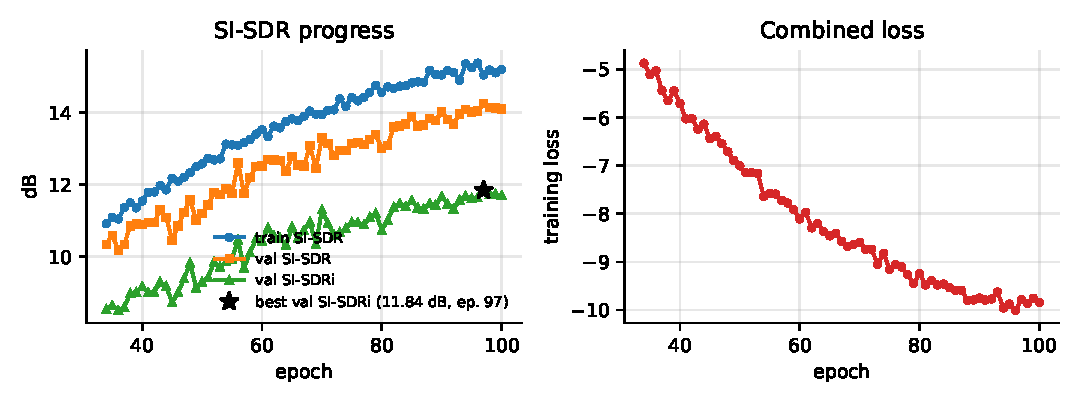
\includegraphics[width=\textwidth]{training_curves.pdf}
\caption{Training behaviour over all 100 epochs, including training loss, training and validation
\sisdr, and validation \sisdri. The best validation \sisdri{} is 11.84\,dB at epoch~97.}
\label{fig:curves}
\end{figure}

\begin{table}[htbp]
\centering\footnotesize
\caption{Selected training milestones from the full 100-epoch log. The complete log is
\texttt{report/data/training\_log.csv}.}
\label{tab:milestones}
\begin{tabular}{@{}r r r r r r@{}}
\toprule
\textbf{Epoch} & \textbf{Train loss} & \textbf{Train \sisdr} & \textbf{Val \sisdr} &
\textbf{Val \sisdri} & \textbf{Learning rate}\\
\midrule
1   & 6.42   & 3.27  & 4.12  & 2.90  & $2.50\times10^{-4}$\\
10  & $-0.29$& 7.60  & 7.32  & 5.77  & $4.92\times10^{-4}$\\
25  & $-3.56$& 9.91  & 9.09  & 7.31  & $4.36\times10^{-4}$\\
33  & $-4.84$& 10.89 & 9.94  & 8.12  & $3.89\times10^{-4}$\\
50  & $-7.01$& 12.57 & 11.20 & 9.29  & $2.63\times10^{-4}$\\
75  & $-9.15$& 14.41 & 13.13 & 10.95 & $8.46\times10^{-5}$\\
90  & $-9.75$& 15.04 & 14.01 & 11.66 & $2.25\times10^{-5}$\\
97  & $-9.79$& 15.04 & 14.24 & \textbf{11.84} & $1.11\times10^{-5}$\\
100 & $-9.84$& 15.19 & 14.10 & 11.69 & $1.00\times10^{-5}$\\
\bottomrule
\end{tabular}
\end{table}

The training loss fell from 6.42 to $-9.84$ and training \sisdr{} rose from 3.27 to 15.19\,dB.
Over the last ten epochs the train--validation \sisdr{} gap averaged about 1.15\,dB, so there is
no strong overfitting. The curve flattens as the learning rate anneals towards $10^{-5}$: from
epoch~90 onward, validation \sisdri{} stayed between 11.32 and 11.84\,dB. No batches were skipped
for non-finite loss. Swings of a few tenths of a dB from epoch to epoch are normal because the
validation set has only 300 mixtures.

\subsection{Test-set metrics}
\label{sec:testmetrics}
\Cref{tab:test} gives \sisdr, STOI and wideband PESQ on the test set with 95\% bootstrap
confidence intervals. The headline row group excludes the 65 clean-scenario items, where the
mixture already equals the reference.

\begin{table}[htbp]
\centering\small
\caption{Test metrics for the epoch-97 checkpoint, mean with 95\% bootstrap CI. The headline
column excludes the 65 clean-scenario items.}
\label{tab:test}
\begin{tabular}{@{}lcc@{}}
\toprule
Metric & Non-clean ($n{=}1135$) & All items ($n{=}1200$)\\
\midrule
\sisdr{} input (dB) & 0.28 [0.00, 0.56] & 5.95 [4.62, 7.33]\\
\sisdr{} output (dB) & 11.92 [11.40, 12.44] & 13.92 [13.22, 14.61]\\
\textbf{\sisdri{} (dB)} & \textbf{11.64 [11.17, 12.09]} & 7.97 [6.99, 8.90]\\
STOI input & 0.772 [0.765, 0.780] & 0.785 [0.777, 0.792]\\
STOI output & 0.882 [0.873, 0.891] & 0.888 [0.879, 0.897]\\
PESQ input (wideband) & 1.33 & 1.51\\
PESQ output (wideband) & 2.38 [2.33, 2.42] & 2.50 [2.45, 2.55]\\
\bottomrule
\end{tabular}
\end{table}

The main conclusions from \Cref{tab:test} are:
\begin{itemize}
  \item \textbf{Enhancement:} On the 1135 non-clean items, SI-SDR improves by 11.64\,dB,
        STOI rises from 0.772 to 0.882, and wideband PESQ rises from 1.33 to 2.38.
  \item \textbf{Why non-clean is the headline:} The all-items SI-SDRi is only 7.97\,dB because
        the 65 clean items have an input SI-SDR of about 105\,dB. Their output SI-SDR of 48.81\,dB
        therefore appears as a $-56$\,dB ``improvement'', which is a metric artefact.
  \item \textbf{Clean speech:} STOI remains 1.00, while PESQ changes only from 4.64 to 4.62,
        showing that clean speech passes through almost unchanged.
\end{itemize}

\begin{table}[htbp]
\centering\small
\caption{Results by scenario for the epoch-97 checkpoint. STOI and PESQ are reported as
input/output.}
\label{tab:scenario}
\begin{tabular}{@{}lrrrrrr@{}}
\toprule
Scenario & $n$ & \sisdr{} in & \sisdr{} out & \sisdri{} [95\% CI] & STOI in/out & PESQ in/out\\
\midrule
noise & 290 & 4.22 & 18.08 & 13.86 [13.17, 14.58] & 0.90/0.95 & 1.75/2.99\\
speech & 294 & 1.15 & 12.08 & 10.92 [9.93, 11.83] & 0.76/0.90 & 1.28/2.54\\
speech\_noise & 551 & $-2.25$ & 8.60 & 10.85 [10.15, 11.52] & 0.71/0.84 & 1.14/1.97\\
clean & 65 & 104.86 & 48.81 & $-56.05$ [$-58.36$, $-54.02$] & 1.00/1.00 & 4.64/4.62\\
\bottomrule
\end{tabular}
\end{table}

Denoising alone (noise scenario) is easiest at 13.86\,dB. Removing a competing talker (speech,
10.92\,dB) and the hardest combination of talker plus noise (speech\_noise, 10.85\,dB) both give
about 11\,dB; the latter has the lowest output STOI (0.84) and PESQ (1.97). The \sisdri{} gain
shrinks as input SNR rises, from about 13\,dB at low SNR to about 10\,dB at high SNR, which is
expected because there is less noise left to remove; absolute quality (PESQ) improves with SNR.
The model does not collapse at hard ratios, and it still gains about 13\,dB at SIR below
$-3.3$\,dB and at SNR below $-1.7$\,dB. Across the 16 DEMAND environments the mean \sisdri{}
ranges from 6.91\,dB (restaurant, \texttt{PRESTO}) to 18.72\,dB (washing, \texttt{DWASHING});
the hardest environments are crowded or transit scenes. The full SIR/SNR and environment
breakdowns are in \Cref{app:breakdowns}.

\subsection{Speaker confusion}
\label{sec:confusion}
The most characteristic TSE failure is extracting the \emph{wrong} speaker. For the 845 test
mixtures that contain an interferer we embedded the output, the clean target and a 5\,s segment of
the interferer with ECAPA-TDNN, and counted an output as confused when it is closer in cosine
similarity to the interferer than to the target. The confusion rate is \textbf{7.7\%} (65 of 845).
Mean similarity to the target rises from 0.584 for the mixture to 0.772 for the output.
\Cref{fig:confusion} (top) shows the two clusters and (bottom) the rate by condition.
\Cref{tab:confusion} gives the rate by enrollment duration.

\begin{figure}[t]
\centering
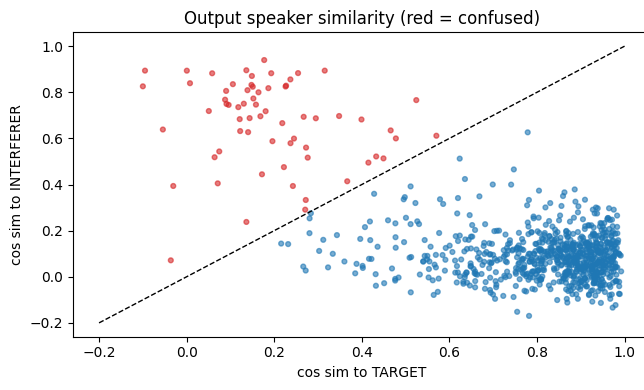
\includegraphics[width=0.62\textwidth]{speaker_similarity.png}\\[4pt]
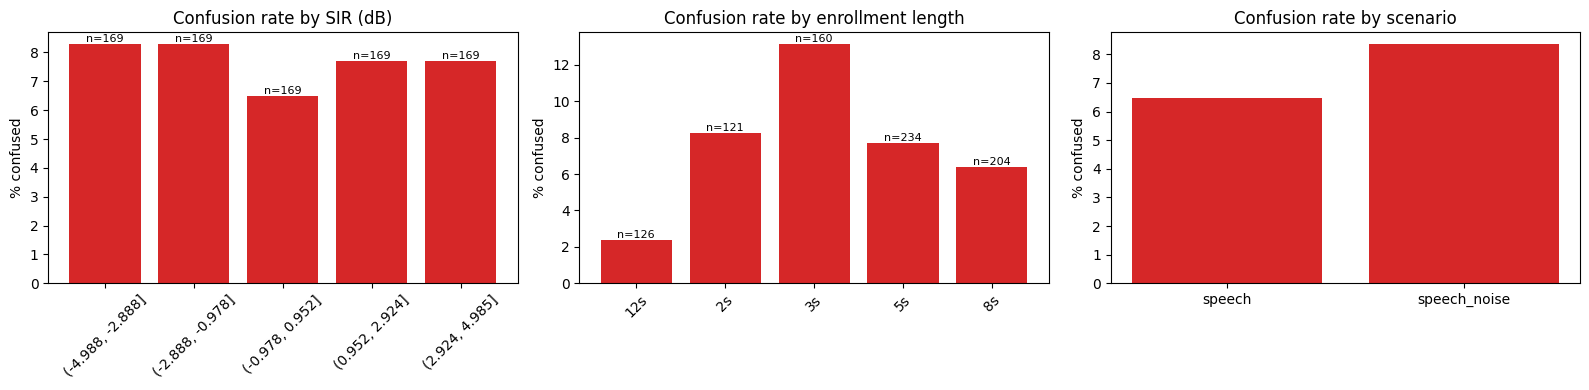
\includegraphics[width=\textwidth]{confusion_drivers.png}
\caption{Top: output similarity to the target versus the interferer (red points are confused
outputs). Bottom: confusion rate by SIR bin, enrollment length and scenario.}
\label{fig:confusion}
\end{figure}

\begin{table}[htbp]
\centering\small
\caption{Speaker-confusion rate by enrollment duration on the 845 interferer test mixtures.}
\label{tab:confusion}
\begin{tabular}{@{}lrrr@{}}
\toprule
Enrollment & $n$ & Confused & Rate\\
\midrule
2\,s & 121 & 10 & 8.3\%\\
3\,s & 160 & 21 & 13.1\%\\
5\,s & 234 & 18 & 7.7\%\\
8\,s & 204 & 13 & 6.4\%\\
12\,s & 126 & 3 & 2.4\%\\
\bottomrule
\end{tabular}
\end{table}

Confusion is roughly independent of SIR (6.5--8.3\%), slightly higher with added noise (8.3\%
versus 6.5\%), and depends on enrollment length. It is lowest with 12\,s enrollments (2.4\%) and
highest with 3\,s enrollments (13.1\%); the trend is not strictly monotonic (2\,s is below 3\,s)
and the 12\,s bin contains only three confusions, so this is suggestive rather than conclusive.
All ten non-clean test mixtures with the lowest \sisdri{} are speaker confusions.

\subsection{Downstream intelligibility}
\label{sec:wer}
To measure usefulness beyond signal metrics, 300 random test mixtures were transcribed with
Whisper \texttt{small.en} \cite{radford2023whisper}, using Whisper's transcript of the \emph{clean
target} as the reference rather than human transcripts, and WER was computed with
\texttt{jiwer}. \Cref{tab:wer} shows that extraction more than halves the WER.

\begin{table}[htbp]
\centering\small
\caption{Whisper WER (\%) on 300 test mixtures from the epoch-97 checkpoint.}
\label{tab:wer}
\begin{tabular}{@{}lrrr@{}}
\toprule
Subset & $n$ & Mixture & Extracted\\
\midrule
All & 300 & 38.3 & \textbf{18.1}\\
Excluding clean & 285 & 40.2 & \textbf{18.9}\\
\midrule
noise & 77 & 7.0 & 5.8\\
speech & 77 & 40.4 & 10.5\\
speech\_noise & 131 & 60.0 & 31.9\\
clean & 15 & 0.0 & 0.0\\
\bottomrule
\end{tabular}
\end{table}

The largest gain is with a competing talker: WER drops from 40.4\% to 10.5\% for speech and from
60.0\% to 31.9\% for speech plus noise. Noise-only mixtures are already easy for Whisper (7.0\%),
and clean speech is not damaged (0\% WER). The relative WER reduction is 52.9\%.

Additional diagnostics use the epoch-97 checkpoint. It improves \sisdr{} on 93.7\% of the 1135
non-clean test mixtures (88.6\% of all 1200, since the 65 clean items cannot improve). On
non-clean items its \sisdri{} correlates weakly and negatively with SNR ($r=-0.19$) and SIR
($r=-0.13$) and is essentially uncorrelated with input \sisdr{} ($r=-0.05$) and enrollment
duration ($r=0.05$). For the 845 mixtures with an interferer, the mean \sisdri{} is 12.84\,dB when
the output matches the target speaker and $-12.67$\,dB when it does not; if the confused outputs
behaved like the correct ones, the non-clean \sisdri{} would rise from 11.64\,dB to 13.10\,dB.

\clearpage
\subsection{Qualitative examples}
Six test mixtures were drawn at random with a fixed seed and listened to. \Cref{tab:examples}
lists \sisdr{} before and after processing with the epoch-97 checkpoint; all six improved by 11.3
to 21.4\,dB. \Cref{fig:spec} shows the spectrograms for the best of the six. These examples are
illustrative and do not replace the statistics above.

\begin{table}[H]
\centering\small
\caption{Randomly chosen test examples from the epoch-97 checkpoint.}
\label{tab:examples}
\begin{tabular}{@{}rrrr@{}}
\toprule
Test index & Input \sisdr{} (dB) & Output \sisdr{} (dB) & Improvement (dB)\\
\midrule
323 & $-3.50$ & 12.27 & $+15.77$\\
761 & 3.80 & 21.57 & $+17.77$\\
611 & 2.52 & 17.88 & $+15.36$\\
369 & $-0.77$ & 20.67 & $+21.44$\\
49 & 1.60 & 12.88 & $+11.27$\\
1016 & $-0.66$ & 11.38 & $+12.04$\\
\bottomrule
\end{tabular}
\end{table}

\begin{figure}[H]
\centering
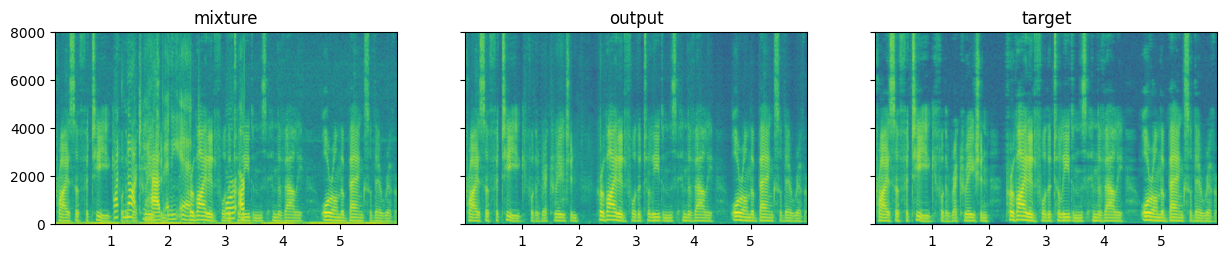
\includegraphics[width=0.88\textwidth]{spec_ex369.png}
\caption{Test example 369 ($+21.4$\,dB, the best of the six): mixture (left), model output
(centre) and clean target (right). The competing voice and broadband noise are removed, and the
output closely resembles the target.}
\label{fig:spec}
\end{figure}

\subsection{Efficiency}
\label{sec:eff}
\Cref{tab:eff} reports inference cost on an NVIDIA L4 for a 6\,s clip, processed offline in one
pass.

\begin{table}[htbp]
\centering\small
\caption{Model size and inference cost for a 6\,s clip, batch 1, on an NVIDIA L4.}
\label{tab:eff}
\begin{tabular}{@{}lrr@{}}
\toprule
 & fp32 & fp16 autocast\\
\midrule
Parameters & \multicolumn{2}{c}{16.83\,M}\\
Compute & \multicolumn{2}{c}{23.87\,GMACs per clip (3.98\,GMACs per second of audio)}\\
Time per clip & 164.9\,ms & 181.1\,ms\\
Offline RTF & 0.0275 & 0.0302\\
Peak GPU memory & 1057\,MiB & 870\,MiB\\
\bottomrule
\end{tabular}
\end{table}

The fp32 pass takes 164.9\,ms for this 6\,s clip; fp16 saves memory but is slower at batch size
one. These are offline GPU measurements. They do not imply low latency: the bidirectional LSTMs
need the whole clip, and CPU speed has not yet been measured.

%% ============================================================
%%  5. LIMITATIONS
%% ============================================================
\section{Challenges and Limitations}
\label{sec:limits}
\begin{itemize}
  \item \textbf{Non-causal model.} Bidirectional LSTMs use future frames, so the current model
        needs the whole utterance and is not suitable for low-latency streaming.
  \item \textbf{Size and compute.} At 16.83\,M parameters and about 4\,GMACs per second of audio,
        the model is larger than a compact CPU-oriented design; CPU latency is still unmeasured.
  \item \textbf{Speaker confusion.} In 7.7\% of interferer mixtures the output matches the
        interferer better than the target, mostly with 2--3\,s enrollments; target-absent
        behaviour is untested.
  \item \textbf{No unseen-noise test.} DEMAND recordings are split by time, so the same 16
        environments appear in training, validation and test; reverberation is also absent.
  \item \textbf{Enrollment mismatch.} Enrollments are VAD-cleaned from clean recordings with only
        10 recipes per training speaker, whereas real enrollments are noisier and less controlled.
  \item \textbf{Evaluation scope.} The validation set has 300 mixtures, and the WER reference is a
        Whisper transcript of the clean target rather than a human transcript.
\end{itemize}

%% ============================================================
%%  6. REMAINING WORK
%% ============================================================
\section{Remaining Work and Revised Plan}
\label{sec:remaining}
The remaining work is organised over eight weeks. It starts with the evaluation gaps that most
affect the validity of the current results, then moves to robustness, deployment and
documentation. \Cref{tab:plan} lists the tasks.

\begin{table}[H]
\centering\small
\caption{Remaining work and revised plan.}
\label{tab:plan}
\begin{tabularx}{\textwidth}{@{}>{\raggedright\arraybackslash}p{4.3cm} Y@{}}
\toprule
\textbf{Task} & \textbf{Description}\\
\midrule
Conditioning ablation & Compare additive-only, FiLM-only and concatenation/gating conditioning
  under identical splits and report \sisdri, STOI and PESQ.\\
Unseen-noise and target-absent evaluation & Hold out whole DEMAND environments, add MUSAN or
  self-recorded noise, and evaluate target-absent and short-enrollment cases.\\
Causal and compact variant & Build a unidirectional-LSTM/causal-STFT variant, reduce the model if
  needed, and measure CPU RTF, latency and memory.\\
Enrollment robustness & Test noisy, reverberant and longer enrollments and quantify the effect on
  speaker confusion.\\
Demo and reproducibility package & Package the inference script, example enrollment, fixed
  configurations and a short usage guide.\\
Final report and presentation & Consolidate all results, refresh tables and figures, and prepare
  the final submission and presentation.\\
\bottomrule
\end{tabularx}
\end{table}

%% ============================================================
%%  7. CONCLUSION
%% ============================================================
\section{Conclusion}
\label{sec:conclusion}
We implemented and trained a speaker-conditioned BSRNN for single-channel target speaker
extraction. The final model contains 16.83\,M parameters, uses a frozen ECAPA-TDNN enrollment
encoder, and injects the speaker vector through additive features and FiLM in eight dual-path
layers. Training completed all 100 epochs and reached a best validation \sisdri{} of 11.84\,dB at
epoch~97 on unseen speakers. On the 1200-mixture test set, the epoch-97 checkpoint improved
non-clean \sisdr{} by 11.64\,dB, raised STOI from 0.772 to 0.882 and PESQ from 1.33 to 2.38, and
reduced Whisper WER from 38.3\% to 18.1\%. The main failure mode is speaker confusion (7.7\% of
interferer mixtures), and the main engineering limitation is that the model is non-causal and has
not yet been measured on CPU. The next phase focuses on conditioning ablation, unseen-noise and
target-absent evaluation, a causal/compact variant and final documentation.

%% ============================================================
%%  REFERENCES
%% ============================================================
\bibliographystyle{ieeetr}
\setlength{\bibsep}{2pt}
\bibliography{references}

%% ============================================================
%%  APPENDIX
%% ============================================================
\appendix

\section{Reproducibility Notes}
\label{app:repro}
\begin{itemize}
  \item \textbf{Result files:} \texttt{test\_metrics.csv} (per-mixture \sisdr, STOI and output
        PESQ), \texttt{pesq\_in.csv} (input PESQ), \texttt{speaker\_confusion.csv} and
        \texttt{wer\_transcripts.csv}, all generated with the epoch-97 checkpoint.
  \item \textbf{Code:} \texttt{tselib.py} contains the model, sampler, datasets, loss and training
        loop, with two YAML configuration files. These are kept on Google Drive under
        \texttt{tse-project/}. The project repository is at
        \url{https://github.com/frecklehead/SIC-AI-Project}.
  \item \textbf{Training notebook:} downloads LibriSpeech and DEMAND, loads manifests and cached
        embedding banks, patches gradient checkpointing, and calls \texttt{T.train(\ldots)}.
  \item \textbf{Test notebook:} loads the best checkpoint, plays the mixture, output and target,
        computes \sisdr, STOI and PESQ on the test manifest, and separates user-supplied files.
  \item \textbf{Software:} PyTorch 2.x (CUDA), SpeechBrain, \texttt{pystoi}, \texttt{pesq},
        \texttt{jiwer} and Whisper through \texttt{transformers} for the WER check.
  \item \textbf{Analysis:} per-scenario, SNR, SIR and noise-environment breakdowns, bootstrap
        confidence intervals, speaker-confusion analysis, WER and FLOP/RTF benchmarking are in the
        analysis cells of the training notebook.
\end{itemize}

\section{Additional Results}
\label{app:breakdowns}

\begin{table}[htbp]
\centering\footnotesize
\caption{\sisdri{} (dB) by difficulty for the epoch-97 checkpoint. SIR bins use the 845 mixtures
with an interferer; SNR bins use the 841 mixtures with noise.}
\label{tab:sirdifficulty}
\begin{tabular}{@{}lrrr@{\hspace{1.2cm}}lrrr@{}}
\toprule
SIR bin (dB) & $n$ & \sisdri{} & PESQ & SNR bin (dB) & $n$ & \sisdri{} & PESQ\\
\midrule
$[-5.0,-3.3]$ & 131 & 12.57 & 1.96 & $[-5.0,-1.7]$ & 155 & 13.24 & 1.86\\
$(-3.3,-1.7]$ & 152 & 10.84 & 2.00 & $(-1.7,1.7]$ & 136 & 13.68 & 2.19\\
$(-1.7,0.0]$ & 134 & 12.23 & 2.14 & $(1.7,5.0]$ & 142 & 12.57 & 2.38\\
$(0.0,1.7]$ & 147 & 10.95 & 2.20 & $(5.0,8.3]$ & 135 & 11.63 & 2.47\\
$(1.7,3.3]$ & 144 & 9.32 & 2.28 & $(8.3,11.6]$ & 126 & 10.38 & 2.48\\
$(3.3,5.0]$ & 137 & 9.52 & 2.41 & $(11.6,14.9]$ & 147 & 9.67 & 2.59\\
\bottomrule
\end{tabular}
\end{table}

\begin{table}[htbp]
\centering\footnotesize
\caption{Mean \sisdri{} and output quality per DEMAND environment for the epoch-97 checkpoint
(all 841 test mixtures that contain noise).}
\label{tab:noiseenv}
\begin{tabular}{@{}lrrrr@{\hspace{0.8cm}}lrrrr@{}}
\toprule
Env. & $n$ & \sisdri{} & STOI & PESQ & Env. & $n$ & \sisdri{} & STOI & PESQ\\
\midrule
DKITCHEN & 57 & 14.95 & 0.93 & 2.74 & OOFFICE & 48 & 13.44 & 0.89 & 2.49\\
DLIVING & 61 & 9.50 & 0.85 & 1.92 & PRESTO & 49 & 6.91 & 0.79 & 1.74\\
DWASHING & 33 & 18.72 & 0.93 & 2.96 & PSTATION & 64 & 8.38 & 0.83 & 2.06\\
NFIELD & 44 & 13.88 & 0.90 & 2.39 & SPSQUARE & 49 & 11.13 & 0.87 & 2.14\\
NPARK & 52 & 11.74 & 0.85 & 2.05 & STRAFFIC & 51 & 11.25 & 0.90 & 2.43\\
NRIVER & 44 & 12.90 & 0.87 & 2.27 & TBUS & 63 & 14.46 & 0.93 & 2.80\\
OHALLWAY & 53 & 13.94 & 0.89 & 2.49 & TCAR & 52 & 15.03 & 0.94 & 3.03\\
OMEETING & 65 & 9.20 & 0.84 & 1.98 & TMETRO & 56 & 8.78 & 0.83 & 1.94\\
\bottomrule
\end{tabular}
\end{table}

\begin{table}[H]
\centering\footnotesize
\caption{Causal Conv-TasNet baseline configuration and result. The saved best checkpoint is
epoch~21.}
\label{tab:convtasnet}
\begin{tabularx}{\textwidth}{@{}lY@{}}
\toprule
Configuration & Causal; $N=512$, $H=512$; film2 conditioning; 3\,s segments; batch 3 with
gradient accumulation 2; learning rate $10^{-3}$; 80 epochs planned\\
Best checkpoint & Epoch 21, validation \sisdri{} 5.90\,dB\\
20-clip check & 3.88\,dB on training voices; 3.60\,dB on held-out voices and noise\\
Decision & Retained as a documented baseline; the final system uses BSRNN\\
\bottomrule
\end{tabularx}
\end{table}

\end{document}
